The history about this term begins near the year 2008 \cite{DefineGamefication}. 
It was coined to summarise the use of game elements on non-game contexts.
In the year 2010 the term reached the critical mass to appear on Google
Trends\cite{LiCap1.3}.

The idea of this concept initially was use on the 80s to make an upgrade to a 
game called MUD \emph{Multy User Dungeons}. The person behind this was Richard Bartle
who begin to analise the people who played this games and found 4 stereotypes of
players,\ref{fig:Players}.

With this types of players he developed a new MUD to satisfy each type of player.
After the sucess of the idea of focus certein aspects of the game to engage the players
the non-game industry began to use game elements to engage people over their products. 

\begin{figure}[!htb]
  \centering
  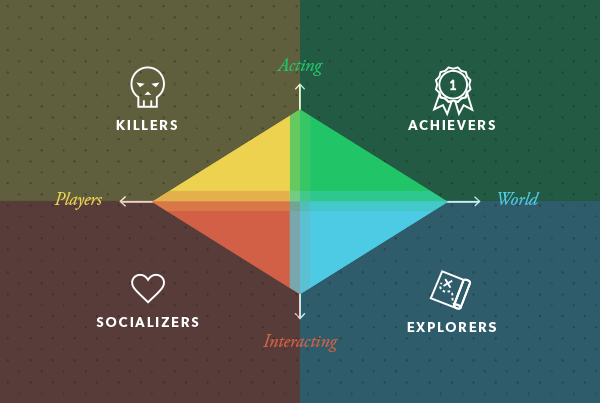
\includegraphics[width=0.5\textwidth]{images/TypeOfPlayersBartle.png}
  \caption[Caption for LOF]{Real caption\footnotemark}
  \label{fig:Players}
\end{figure}

\footnotetext{Source: \url{http://www.example.com/theimage.png}}
 	

Nowadays Gamification has become a really useful tool to engage people. With this in
mind the industry and people are in the need of a description that can contain
all the ideas about it. \emph{Gamification} is \emph{the use of game design elements
in non-game related contexts}:

\begin{itemize}

\item Game: This relates to \emph{games} and not to \emph{play}. The idea of game is
characterized by explicit rules that make a context where the competition or strife
of actors let them go towars goals or achievements.    

\item Game elements: Within this concept there are two definitions. The first,
only accept certain unique elements. This is a very constraint approach were the set
of useful elements is a very tight. The other definition is a boundless one were every
element from every game can be use. With this two ideas we can create a more restrict 
definition were the elements to use are characteristic to games, that are
found in most (but not necessarily all) games, found to play a significant role in gameplay. 

\item Design: 

\begin{table}[h]
  \begin{center}
    \begin{tabular}{ | p{5cm} | p{5cm} | p{5cm} |}
    \hline
    Level & Description &  Example \\ \hline
    \emph{Game interface design patterns}. & 
    Common, successful interaction
    design components and design
    solutions for a known problem in
    a context, including prototypical
    implementations. &
    Badge, leaderboard, level. \\ \hline
    Game design patterns and
    mechanics. & 
    Commonly reoccurring parts of
    the design of a game that concern
    gameplay. &
    Time constraint,
    limited resources,
    turns. \\ \hline
    Game design principles and
    heuristics &
    Evaluative guidelines to approach
    a design problem or
    analyze a given design solution &
    Enduring play, clear goals, variety of
    game styles \\ \hline
    Game models &
    Conceptual models of the
    components of games or game
    experience &
    MDA; challenge,
    fantasy, curiosity;
    game design atoms;
    CEGE \\ \hline
    Game design methods &
    Game design-specific practices
    and processes &
    Playtesting, playcentric design,
    value conscious game design \\ \hline
    \end{tabular}
    \caption[]{\cite{DefineGamefication}}
  \end{center}
\end{table}
\item Non-Game Context:

\end{itemize}

Gamification can be use on multiple context where the attention of the user is needed. Some of this context are education, sales and marketing.

\begin{itemize}

\item Education: In this context the use of gamification can be seen in different ideas to engage the
the students and keep them interested. Some of this concepts can be use in schools and universities
where the students are 

\item Sales and marketing:

\end{itemize}

